Dado el sistema

\begin{equation}
    G(s) = a\frac{(s - b)}{s(s-c)(s-d)}
\end{equation}

\noindent se identifica lo siguiente:
\begin{itemize}
    \item Ceros: $b$
    \item Polos: $0, c$ y $d$
    \item Ganancia: $a$
\end{itemize}


\noindent Además, $a$ y $b$ se definen mediante:

\begin{equation*}
    a = -\frac{cd}{b} \qquad b = \frac{c + d}{2}
\end{equation*}

La Figura \ref{fig:1} muestra la entrada escalón unitario y la correspondiente salida del sistema $G$

\begin{figure}[ht!]
    \centering
    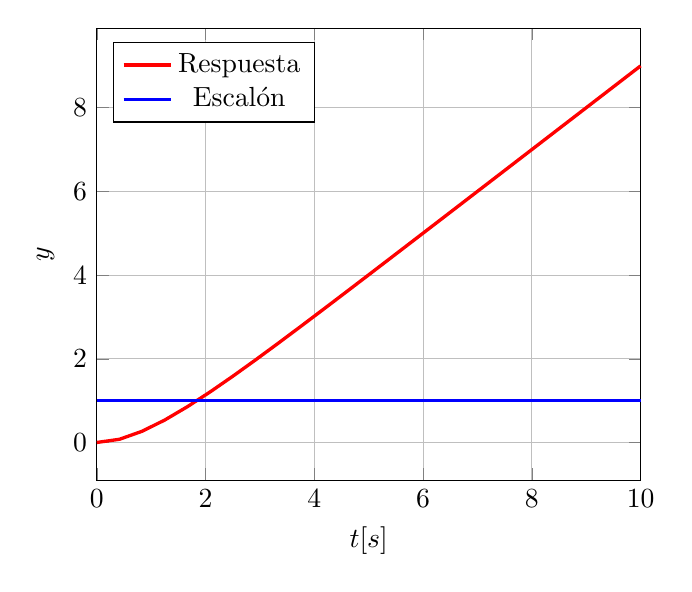
\begin{tikzpicture}
        \begin{axis}[
            width = 0.7\textwidth,
            xmin = 0, xmax = 10,
            grid = both,
            clip = false,
            xlabel = {$t [s]$},
            ylabel = {$y$},
            legend entries = {Respuesta, Escalón},
            legend pos = north west
        ]
            \addplot[domain = 0:10, red, very thick]{x + exp(-x) - 1};
            \addplot[domain = 0:10, blue, very thick]{1};
        \end{axis}
    \end{tikzpicture}
    \caption{Respuesta del sistema $G(s)$ ante una entrada escalón}
    \label{fig:1}
\end{figure}


Para entender porqué la respuesta del sistema es lineal, primero veamos la función de transferencia $G(s)$. La función de transferencia se define como la razón entre la salida y la entrada al sistema, es decir

\begin{equation}
    \frac{C(s)}{R(s)} = G(s),
\end{equation}

\noindent siendo $R$ y $C$ la entrada y salida del sistema respectivamente. Reordenemos la expresión:

\begin{equation*}
    C(s) = G(s)R(s)   
\end{equation*}



\noindent Dado que la entrada al sistema es una función de Heaviside, entonces $R(s) = 1/s$. Por lo tanto, la salida del sistema queda expresado como el producto entre la función de transferencia y la salida del sistema en el dominio complejo. Para obtener una expresión en el tiempo (lo que buscamos), necesitamos aplicar la transformada inversa de Laplace. Por lo tanto:

\begin{equation}
    \label{eq:3}
    c(t) = y(t) = \mathcal{L}^{-1} [G(s)R(s)] = \mathcal{L}^{-1} \left[a\frac{(s - b)}{s(s-c)(s-d)} \frac{1}{s}\right] 
\end{equation}



La expresión \ref{eq:3} se puede resolver mediante técnica de fracciones parciales o convolución, pero se puede utilizar la función integrada de Matlab \texttt{ilaplace()} para calcular su inversa. La expresión encontrada es:

\begin{equation}
    y(t) = t + e^{-t} - 1
\end{equation}


\noindent Se observa que para el término exponencial es cada vez más chico a medida que $t$ crece, prevaleciendo el término dominante de la expresión: $y(t) = t$. Esta es la razón por la que el sistema presenta una recta como respuesta.


Volvamos a la función de transferencia $G(s)$. Claramente el sistema es inestable pero hay una manera de estabilizar el sistema. Podemos aplicar el \textbf{Teorema del valor final} a $C(s)$, entonces:

\begin{equation}
    \lim_{t \to \infty} c(t) = \lim_{s \to 0} sG(s)R(s) = \lim_{s \to 0} s a\frac{(s - b)}{s(s-c)(s-d)} \frac{1}{s} = +\infty
\end{equation}


\noindent Es decir, el integrador $1/s$ es el responsable de que el sistema diverga. Por lo tanto, sacando el integrador de $G(s)$, se obtiene lo siguiente:

\begin{equation}
    \label{eq:6}
    \lim_{s \to 0} s \underbrace{a\frac{(s - b)}{(s-c)(s-d)}}_{G(s) \ \text{sin el integrador}} \frac{1}{s} = -\frac{ab}{cd}
\end{equation}


En la Figura \ref{fig:2} se observa el comportamiento del sistema ante la entrada escalón cuando $G$ no tiene el integrador.

\begin{figure}[ht!]
    \centering
    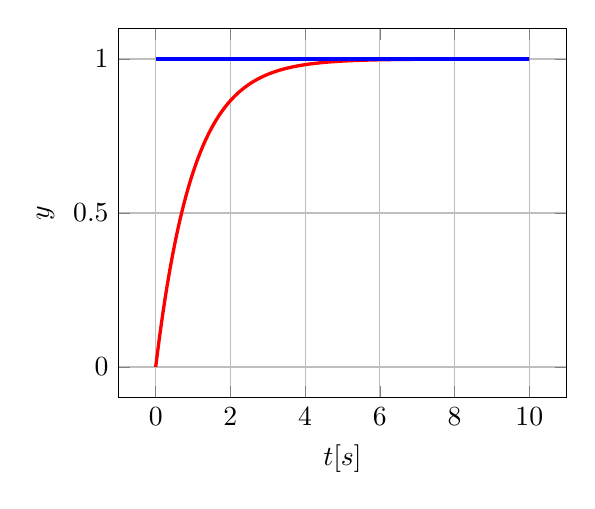
\begin{tikzpicture}
        \begin{axis}[
            width = 0.6\textwidth,
            grid = both,
            xlabel = {$t [s]$},
            ylabel = {$y$}
        ]
            \addplot[red, very thick, domain = 0:10, samples = 200]{1 - exp(-x)};
            \addplot[blue, very thick, domain = 0:10]{1};
        \end{axis}
    \end{tikzpicture}
    \caption{Función transferencia $G(s)$ sin integrador}
    \label{fig:2}
\end{figure}



Se observa en la gráfica \ref{fig:2} que no hay sobrepaso en la respuesta. La razón de esto se debe a los polos de la función transferencia únicamente tienen parte real negativa. En la Figura \ref{fig:3} se grafican 4 respuestas con distintos valores de los polos.

El sistema original tiene polos $-1\pm i$. Para calcular el sobrepaso se hace uso de la siguiente expresión:

\begin{equation}
    M_p = \frac{|y_{\text{máx}} - y_{\text{end}}|}{y_{\text{end}}}100
\end{equation}

\noindent donde $y_{\text{end}}$ es la expresión \ref{eq:6}. Por lo tanto, el sobrepaso $M_p$ de mi sistema es:

\begin{equation}
    M_p = \frac{|1.20788 - 1|}{1}100 = 20.788\%
\end{equation}

Claramente si aumentamos la magnitud de la parte imaginaria de los polos el sobrepaso será mucho más grande.

\begin{figure}[ht!]
    \centering
    \begin{tikzpicture}
        \begin{groupplot}[group style = {group size = 2 by 2,
            horizontal sep=1.8cm,
            vertical sep=1.8cm},
            width=7cm, height=6cm,
            ylabel={$y(t)$},
            grid = both,
            trig format = rad,
            ylabel style = {rotate = -0.46},
            ]
            %-----PRIMER SUBPLOT----- c = -1, d = -1
            \nextgroupplot[title = {$c = d = -1$}]
            \addplot[domain = 0:10, black, very thick, samples = 200]{1-exp(-x)};
            %-----SEGUNDO SUBPLOT----- c = -4, d = -5
            \nextgroupplot[ylabel = \empty, title = {$c = -4, d = -5$}]
            \addplot[domain = 0:10, black, very thick, samples = 200]{1 - (4*exp(-5*x))/9 - (5*exp(-4*x))/9};
            %-----TERCER SUBPLOT----- c = -1+i, d = -1-i
            \nextgroupplot[title = {$c,d = -1\pm i$}, xlabel = {$t[s]$}]
            \addplot[domain = 0:10, black, very thick, samples = 200]{1-exp(-x)*(cos(x) - sin(x))};
            %-----CUARTO SUBPLOT----- c = -1 + 3i, d = -1-3i
            \nextgroupplot[ylabel = \empty, title = {$c,d = -1\pm 3i$}, xlabel = {$t[s]$}]
            \addplot[domain = 0:10, black, very thick, samples = 200]{1-exp(-x)*(cos(3*x) - 3*sin(3*x))};
        \end{groupplot}
    \end{tikzpicture}
    \caption{Respuestas del sistema ante la variación de los polos. Para polos reales y negativos la respuesta es totalmente sobreamortiguada, no existe un sobrepaso. Cuando los polos son complejos conjugados existe un sobrepaso en la respuesta. A medida que la parte imaginaria se hace más grande en magnitud, más grande es el sobrepaso.}
    \label{fig:3}
\end{figure}



Por último, veamos la función \texttt{stepinfo(sys)}. Dicha función permite calcular características de respuesta al escalón para un modelo de sistema dinámico o para un arreglo de datos de respuesta al escalón\footnote{\url{https://la.mathworks.com/help/control/ref/dynamicsystem.stepinfo.html}}. Algunas de estas características son:

\begin{multicols}{3}
    \begin{itemize}
        \item \texttt{RiseTime}
        \item \texttt{TransientTime}
        \item \texttt{SettlingTime}
        \item \texttt{SettlingMin}
        \item \texttt{SettlingMax}
        \item \texttt{Overshoot}
        \item \texttt{Undershoot}
        \item \texttt{Peak}
        \item \texttt{PeakTime}
    \end{itemize}
\end{multicols}


\newpage

En la Figura \ref{fig:4} se muestra visualmente estas características del sistema y la Código \ref{cod:1} de Matlab usado para cada punto de esta guía.

\begin{figure}[ht!]
    \centering
    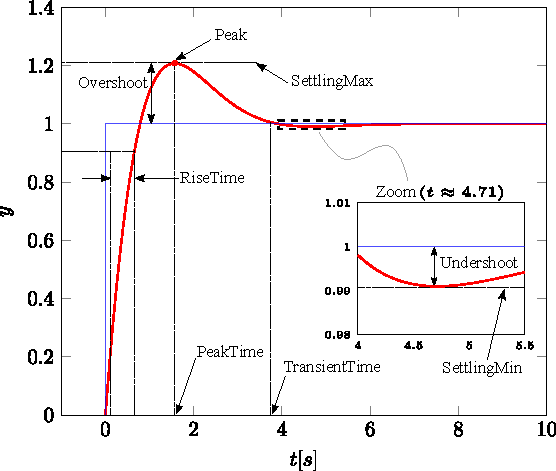
\includegraphics[width=0.8\textwidth]{imagenes/infostepG.pdf}
    \caption{Características del sistema ante la respuesta escalón. El \texttt{RiseTime} es el tiempo que tarda la respuesta en subir del $10\%$ al $90\%$. El \texttt{TransientTime} es el primer tiempo tal que el error está por debajo del $2\%$. Las demás características se pueden deducir fácilmente.}
    \label{fig:4}
\end{figure}



\begin{figure}[ht!]
    \begin{lstlisting}[caption = {Código Matlab hecho para la guía 05.}, label = {cod:1}]
        %%% Parámetros de la función transferencia
    c = -1+i; %Tiene que ser negativo para asegurar la negatividad de los polos. Si pongo polos complejos
    %conjugados hay sobrepaso
    d = -1-i;
    b = (c+d)/2;
    a = -c*d/b;

    %%% Extraigo la información del simulink
    var = sim('Curso_Matlab\semana3\ceros_polos1.slx'); %Si saco el factor 1/s el sistema se estabiliza
    data = var.yout.extractTimetable;
    t = data.Data; escalon = data.Data_1 ; salida = data.Data_2;
    figure();
    plot(t, salida, 'r');
    hold on;
    plot(t, escalon, 'b');

    %%

    %%% Corroboramos porqué es una función lineal
    syms s
    Gs = a*(s-b)/((s-c)*(s-d));
    Hs = 1/s; %entrada escalón unitaria
    gt = ilaplace(Gs*Hs);

    %%

    %%% Cálculo del sobrepaso
    yFinal = -a*b/(c*d);
    yEnd = salida(end);
    display(yEnd)
    display(yFinal)

    maxY = max(salida); %para el sobrepaso
    fprintf('El máximo es: %f\n', maxY);
    sobrepaso = 100*abs(maxY - yFinal) / yFinal;
    fprintf('El sobrepaso en porcentaje es: %.3f \n', sobrepaso);

    %%

    %%% Función zpk y Overshoot
    ceros = [b];
    polos = [c d];
    ganancia = a;
    G = zpk(ceros, polos, ganancia);
    infoG = stepinfo(G);
    \end{lstlisting}
\end{figure}
